\documentclass[fleqn]{article}
\oddsidemargin 0.0in
\textwidth 6.0in
\thispagestyle{empty}
\usepackage{import}
\usepackage{amsmath}
\usepackage{graphicx}
\usepackage{flexisym}
\usepackage{calligra}
\usepackage{amssymb}
\usepackage{bigints} 
\usepackage[english]{babel}
\usepackage[utf8x]{inputenc}
\usepackage{float}
\usepackage[colorinlistoftodos]{todonotes}


\DeclareMathAlphabet{\mathcalligra}{T1}{calligra}{m}{n}
\DeclareFontShape{T1}{calligra}{m}{n}{<->s*[2.2]callig15}{}
\newcommand{\scriptr}{\mathcalligra{r}\,}
\newcommand{\boldscriptr}{\pmb{\mathcalligra{r}}\,}

\definecolor{hwColor}{HTML}{1a0252}

\begin{document}

  \begin{titlepage}

    \newcommand{\HRule}{\rule{\linewidth}{0.5mm}}

    \center


    \textsc{\LARGE Arizona State University}\\[1.5cm]

    \textsc{\LARGE Classical Parts/Field/Matter II}\\[1.5cm]


    \begin{figure}
      
\includegraphics[width=\linewidth]{asu.png}
    \end{figure}


    \HRule \\[0.4cm]
    { \huge \bfseries Problem Set 1}\\[0.4cm] 
    \HRule \\[1.5cm]

    \textbf{Behnam Amiri}

    \bigbreak

    \textbf{Prof: Maulik Parikh}

    \bigbreak


    \textbf{{\large \today}\\[2cm]}

    \vfill

  \end{titlepage}

  \begin{enumerate}
    \item If a charge is located at the coordinates $(2, -2, 1)$ and we are interested
    in some field at the point $(6, 3, 2)$, write down (in our and Griffiths’ notation)

      \textcolor{hwColor}{
        \hspace{10pt} Let's recall that a source point, $r^'$, is where an electric charge is located, and a field point, $r$, is which we
        are calculating the electric or magnetic field.
        \\
        \\
        Also, remember that 
        $
          \begin{cases}
            \overrightarrow{r} \equiv x \hat{x}+y \hat{y}+z \hat{z}
            \\
            \\
            \overrightarrow{\scriptr} \equiv r-r^'
            \\
            \\
            r=\sqrt{x^2+y^2+z^2}
          \end{cases}
        $
        \\
        \\
        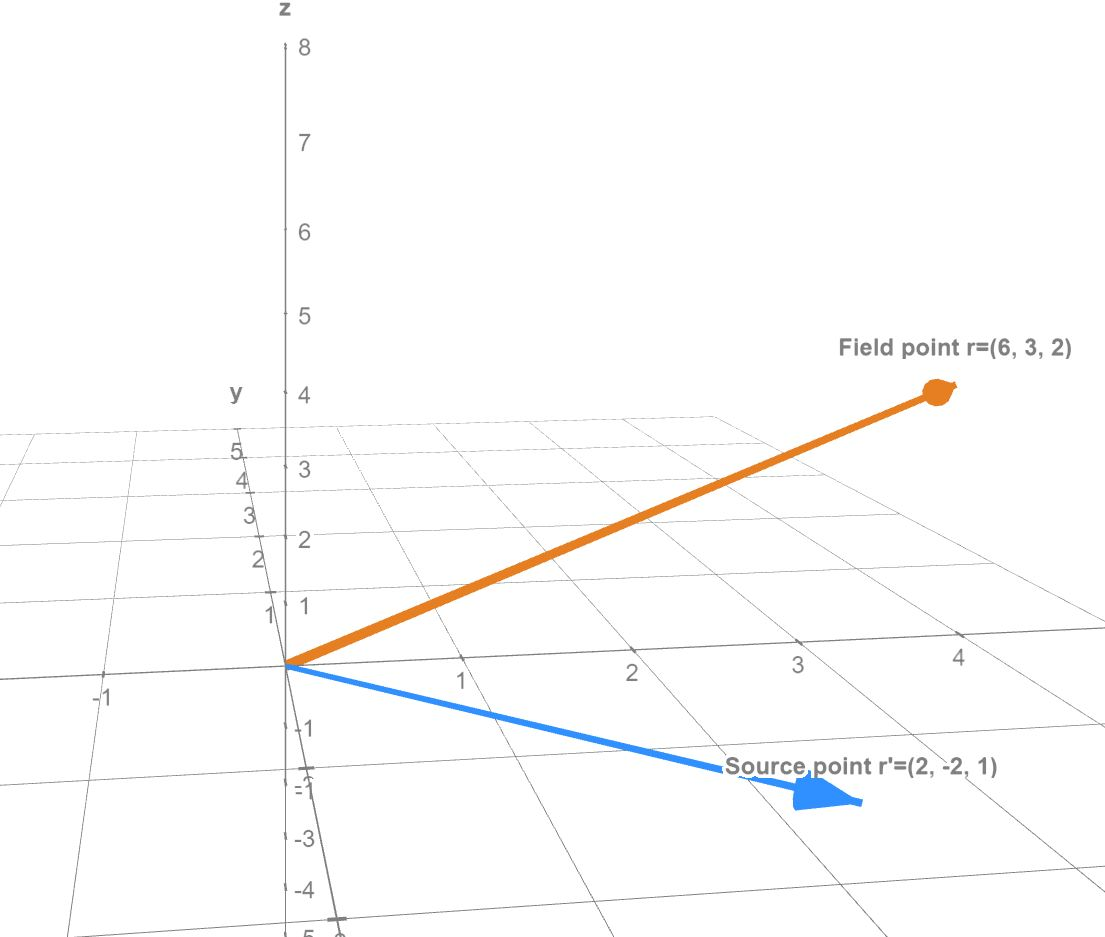
\includegraphics[height=8cm, width=8cm]{A.JPG}
      }
      

    \begin{enumerate}
      \item $\overrightarrow{r}$
      
        \textcolor{hwColor}{
          $
            \overrightarrow{r}=6 \hat{x}+3 \hat{y}+2 \hat{z}
          $
          \\
          \\
        }

      \item $\overrightarrow{r}^'$
      
        \textcolor{hwColor}{
          $
            \overrightarrow{r}^'=2 \hat{x}-2 \hat{y}+\hat{z}
            \\
            \\
          $
        }

      \item $\overrightarrow{\scriptr}$

        \textcolor{hwColor}{
          $
            \overrightarrow{\scriptr}=r-r^'=\left[ 
              \left(6 \hat{x}+3 \hat{y}+2 \hat{z}\right)-\left(2 \hat{x}-2 \hat{y}+\hat{z}\right)
            \right]
            \\
            \\
            \therefore ~~~ \overrightarrow{\scriptr}=4 \hat{x}+5 \hat{y}+\hat{z} 
          $
          \\
          \\
        }

      \item $r$

        \textcolor{hwColor}{
          $
            r=\sqrt{6^2+3^2+2^2}=\sqrt{49}
            \\
            \\
            \therefore ~~~ r=7
          $
          \\
          \\
        }
      
      \item $r^'$

        \textcolor{hwColor}{
          $
            r^'=\sqrt{2^2+(-2)^2+1^2}=\sqrt{9}
            \\
            \\
            \therefore ~~~ r^'=3
          $
        }

      \item $\scriptr$

        \textcolor{hwColor}{
          $
            \scriptr=|r-r^'|=\sqrt{4^2+5^2+1^2}
            \\
            \\
            \therefore ~~~ \scriptr=\sqrt{42}
          $
          \\
          \\
        }

      \item $\hat{r}$

        \textcolor{hwColor}{
          $
            \hat{r}=\dfrac{\overrightarrow{r}}{r}=\dfrac{6 \hat{x}+3 \hat{y}+2 \hat{z}}{7}
            \\
            \\
            \therefore ~~~ \hat{r}=\dfrac{6}{7} \hat{x}+\dfrac{3}{7} \hat{y}+\dfrac{2}{7} \hat{z}
          $
          \\
          \\
        }

      \item $\hat{r}^'$

        \textcolor{hwColor}{
          $
            \hat{r}^'=\dfrac{\overrightarrow{r}^'}{r^'}=\dfrac{2 \hat{x}-2 \hat{y}+\hat{z}}{3}
            \\
            \\
            \therefore ~~~ \hat{r}^'=\dfrac{2}{3} \hat{x}-\dfrac{2}{3} \hat{y}+\dfrac{1}{3}\hat{z}
          $
          \\
          \\
        }

      \item $\hat{\scriptr}$
      
        \textcolor{hwColor}{
          $
            \hat{\scriptr}=\dfrac{\overrightarrow{\scriptr}}{\scriptr}
            =\dfrac{4 \hat{x}+5 \hat{y}+\hat{z} }{\sqrt{42}}
            \\
            \\
            \therefore ~~~ \hat{\scriptr}=\dfrac{4}{\sqrt{42}} \hat{x}+\dfrac{5}{\sqrt{42}} \hat{y}+\dfrac{1}{\sqrt{42}} \hat{z} 
          $
          \\
          \\
        }

    \end{enumerate}

    \item Show that
    \begin{enumerate}
      \item $\overrightarrow{\nabla} \left(\dfrac{1}{\scriptr}\right)=-\dfrac{\hat{\scriptr}}{\scriptr^2}$

        \textcolor{hwColor}{
          $
            \overrightarrow{\nabla} \left(\dfrac{1}{\scriptr}\right)
            =\overrightarrow{\nabla} \left(\dfrac{1}{r-r^'}\right)
            =\overrightarrow{\nabla} \left(\dfrac{1}{\sqrt{(x-x^')^2+(y-y^')^2+(z-z^')^2}}\right)
            \\
            \\
            =\left(\dfrac{\partial}{\partial x} \hat{x}+\dfrac{\partial}{\partial y} \hat{y}+\dfrac{\partial}{\partial z} \hat{z}\right)
            .\left((x-x^')^2+(y-y^')^2+(z-z^')^2\right)^{-\dfrac{1}{2}}
            \\
            \\
            \\
            =\dfrac{\partial}{\partial x} \left((x-x^')^2+(y-y^')^2+(z-z^')^2\right)^{-\dfrac{1}{2}} \hat{x}
            \\
            +\dfrac{\partial}{\partial y} \left((x-x^')^2+(y-y^')^2+(z-z^')^2\right)^{-\dfrac{1}{2}} \hat{y}
            \\
            +\dfrac{\partial}{\partial z} \left((x-x^')^2+(y-y^')^2+(z-z^')^2\right)^{-\dfrac{1}{2}} \hat{z}
            \\
            \\
            \\
            =(-\dfrac{1}{2}) \left((x-x^')^2+(y-y^')^2+(z-z^')^2\right)^{-\dfrac{3}{2}} \dfrac{d}{dx} \left((x-x^')^2+(y-y^')^2+(z-z^')^2\right) \hat{x}
            \\
            +(-\dfrac{1}{2}) \left((x-x^')^2+(y-y^')^2+(z-z^')^2\right)^{-\dfrac{3}{2}} \dfrac{d}{dy} \left((x-x^')^2+(y-y^')^2+(z-z^')^2\right) \hat{y}
            \\
            +(-\dfrac{1}{2}) \left((x-x^')^2+(y-y^')^2+(z-z^')^2\right)^{-\dfrac{3}{2}} \dfrac{d}{dz} \left((x-x^')^2+(y-y^')^2+(z-z^')^2\right) \hat{z}
            \\
            \\
            \\
            =(-\dfrac{1}{2}) \left((x-x^')^2+(y-y^')^2+(z-z^')^2\right)^{-\dfrac{3}{2}} 2(x-x^') \hat{x}
            \\
            +(-\dfrac{1}{2}) \left((x-x^')^2+(y-y^')^2+(z-z^')^2\right)^{-\dfrac{3}{2}} 2(y-y^') \hat{y}
            \\
            +(-\dfrac{1}{2}) \left((x-x^')^2+(y-y^')^2+(z-z^')^2\right)^{-\dfrac{3}{2}} 2(z-z^') \hat{z}
            \\
            \\
            \\
            =-\dfrac{x-x^'}{\left((x-x^')^2+(y-y^')^2+(z-z^')^2\right)^{\dfrac{3}{2}}} \hat{x}
            \\
            -\dfrac{y-y^'}{\left((x-x^')^2+(y-y^')^2+(z-z^')^2\right)^{\dfrac{3}{2}}} \hat{y}
            \\
            -\dfrac{z-z^'}{\left((x-x^')^2+(y-y^')^2+(z-z^')^2\right)^{\dfrac{3}{2}}} \hat{z}
            \\
            \\
            \\
            =-\dfrac{\left[(x-x^')^2 \hat{x}+(y-y^')^2 \hat{y}+(z-z^')^2 \hat{z}\right]}{\sqrt{(x-x^')^2+(y-y^')^2+(z-z^')^2} . \left((x-x^')^2+(y-y^')^2+(z-z^')^2\right)}
            \\
            \\
            \\
            =-\dfrac{\dfrac{(x-x^')^2 \hat{x}+(y-y^')^2 \hat{y}+(z-z^')^2 \hat{z}}{\sqrt{(x-x^')^2+(y-y^')^2+(z-z^')^2}}}{(x-x^')^2+(y-y^')^2+(z-z^')^2}
            \\
            \\
            \\
            \therefore ~~~ \overrightarrow{\nabla} \left(\dfrac{1}{\scriptr}\right)=-\dfrac{\hat{\scriptr}}{\scriptr^2}
            \\
            \\
          $ 
        }

      \item $\overrightarrow{\nabla} . \left(\dfrac{\hat{\scriptr}}{\scriptr^2}\right)=4 \pi \delta^3 (\overrightarrow{\scriptr})$

        \textcolor{hwColor}{
          $
            \overrightarrow{\nabla} . \left(\dfrac{\hat{\scriptr}}{\scriptr^2}\right)
            =\overrightarrow{\nabla} . \left(\dfrac{\dfrac{\overrightarrow{\scriptr}}{\scriptr}}{\scriptr^2}\right)
            =\overrightarrow{\nabla} . \left(\dfrac{\overrightarrow{\scriptr}}{\scriptr^3}\right)
            \\
            \\
            \\
            =\overrightarrow{\nabla} . \left(\dfrac{\overrightarrow{\scriptr}}{\scriptr^3}\right)
            =\left(\dfrac{\partial}{\partial x} \hat{x}+\dfrac{\partial}{\partial y} \hat{y}+\dfrac{\partial}{\partial z} \hat{z}\right)
            . \left(\dfrac{(x-x^') \hat{x}+(y-y^') \hat{y}+(z-z^') \hat{z}}{\left[(x-x^')^2+(y-y^')^2+(z-z^')^2\right]^{3/2}}\right)
            \\
            \\
            \\
            =\dfrac{\partial}{\partial x} \dfrac{(x-x^')}{\left[(x-x^')^2+(y-y^')^2+(z-z^')^2\right]^{3/2}}
            \\
            +\dfrac{\partial}{\partial y} \dfrac{(y-y^')}{\left[(x-x^')^2+(y-y^')^2+(z-z^')^2\right]^{3/2}}
            \\
            +\dfrac{\partial}{\partial z} \dfrac{z-z^'}{\left[(x-x^')^2+(y-y^')^2+(z-z^')^2\right]^{3/2}}
          $
          \\
          \\
          \\
          Let's define $k=(x-x^')^2+(y-y^')^2+(z-z^')^2$ so we have;
          \\
          \\
          $
            =\dfrac{\partial}{\partial x} \dfrac{(x-x^')}{k^{3/2}}
            +\dfrac{\partial}{\partial y} \dfrac{(y-y^')}{k^{3/2}}
            +\dfrac{\partial}{\partial z} \dfrac{(z-z^')}{k^{3/2}}
            \\
            \\
            \\
            =\dfrac{k^{3/2}-\left[\dfrac{3}{2} k^{1/2} \times 2(x-x^')\right] (x-x^')}{k^3}
            +\dfrac{k^{3/2}-\left[\dfrac{3}{2} k^{1/2} \times 2(y-y^')\right] (y-y^')}{k^3}
            +\dfrac{k^{3/2}-\left[\dfrac{3}{2} k^{1/2} \times 2(z-z^')\right] (z-z^')}{k^3}
            \\
            \\
            \\
            =\dfrac{
              \left[k^{3/2} -3(x-x^')^2 k^{1/2}\right]
              +\left[k^{3/2} -3(y-y^')^2 k^{1/2}\right]
              +\left[k^{3/2} -3(y-y^')^2 k^{1/2}\right]
            }{k^3}
            \\
            \\
            \\
            =\dfrac{3k^{3/2}-3k^{1/2} \left((x-x^')^2+(y-y^2)^2+(z-z^')^2\right)}{k^3}
            =\dfrac{3k^{3/2}-\left(3k^{1/2} \times k\right)}{k^3}=0
            \\
            \\
            \\
            \therefore ~~~ \overrightarrow{\nabla} . \left(\dfrac{\hat{\scriptr}}{\scriptr^2}\right)=0
          $
          \\
          \\
          Isn't the result odd?
          \\
          \\
          The given question has $\scriptr$ in the denominator so we do not know the divergence at the origin. Now let's apply the fundamental
          theorem for divergence for a sphere of radius $R$;
          \\
          \\ 
          $
            \bigints\limits_{Volume} \left( \overrightarrow{\nabla} . \overrightarrow{V} \right) d\tau
            =\bigoint\limits_{Surface} \overrightarrow{V} . d\overrightarrow{a}
            =\bigoint\limits_{Surface} \dfrac{1}{R^2} \hat{\scriptr} . \left(R^2 sin(\theta) d\theta d\phi  \hat{\scriptr} \right)
            \\
            \\
            \\
            =\bigoint\limits_{Surface} sin(\theta) d\theta d\phi
            =\bigints\limits_{\theta=0}^{\theta=\pi} sin(\theta) d\theta \bigints\limits_{\phi=0}^{\phi=2\pi} d\phi
            =-cos(\theta) \Big|_{\theta=0}^{\theta=\pi} \times \phi \Big|_{\phi=0}^{\phi=2 \pi}
            =(-1-1) \times 2 \pi=4 \pi
            \\
            \\
            \\
            \therefore ~~~  \bigints\limits_{Volume} \left( \overrightarrow{\nabla} . \overrightarrow{V} \right) d\tau
            =\bigoint\limits_{Surface} \overrightarrow{V} . d\overrightarrow{a}=4 \pi
          $
          \\
          \\
          We found the flux through the sphere of radius $R$. This is suprising! The divergence we calculated was zero but the flux is $4 \pi$.
          Problems liek this one spur the invention of the \textbf{Dirac Delta} function. From page $50$ of the textbook we have;
          \\
          \\
          $$
            \delta^3(r)=\delta(x)\delta(y)\delta(z)
          $$
          The three-dimensional delta function is zero everywhere excpet at $(0, 0, 0)$, where it blows up. Its volume integral is $1$:
          \\
          \\
          $
            \bigints\limits_{all ~ space} \delta^3(r)
            =\bigints\limits_{-\infty}^{+\infty} \bigints\limits_{-\infty}^{+\infty} \bigints\limits_{-\infty}^{+\infty} \delta(x)\delta(y)\delta(z) dx dy dz=1
          $
          \\
          \\
          Now we are in a position to resolve the paradox introduced here. We found that the divergence is zero everywhere excpet at the origin, and yet its
          integral over any volume containing the origin is a constant ($4 \pi$). These are precisely the defining conditions for the \textbf{Dirac Delta}
          function; evidently
          $$
            \overrightarrow{\nabla} . \left(\dfrac{\hat{\scriptr}}{\scriptr^2}\right)=4 \pi \delta^3(\scriptr)
          $$ 
        }

      \item $\overrightarrow{\nabla} \times \scriptr^n \hat{\scriptr}=\overrightarrow{0}$

        \textcolor{hwColor}{
          $
            \overrightarrow{\nabla} \times \scriptr^n \hat{\scriptr}
            =\overrightarrow{\nabla} \times \left(\scriptr^n \dfrac{\overrightarrow{\scriptr}}{\scriptr}\right)
            =\overrightarrow{\nabla} \times \left(\scriptr^{n-1} \overrightarrow{\scriptr}\right)
            \\
            \\
            =\overrightarrow{\nabla} \times \left[\scriptr^{n-1} \left((x-x^') \hat{x}+(y-y^') \hat{y}+(z-z^') \hat{z}\right)\right]
            \\
            \\
            =\begin{vmatrix}
              \hat{x} & \hat{y} & \hat{z} 
              \\
              \\
              \dfrac{\partial}{\partial x} & \dfrac{\partial}{\partial y} & \dfrac{\partial}{\partial z}
              \\
              \\
              \scriptr^{n-1}(x-x^') & \scriptr^{n-1}(y-y^') & \scriptr^{n-1}(z-z^')
            \end{vmatrix}
            \\
            \\
            \\
            =\left[\dfrac{\partial}{\partial y} \scriptr^{n-1}(z-z^')-\dfrac{\partial}{\partial z} \scriptr^{n-1}(y-y^')\right] \hat{x}
            \\
            +\left[\dfrac{\partial}{\partial x} \scriptr^{n-1}(z-z^')-\dfrac{\partial}{\partial z} \scriptr^{n-1}(x-x^')\right] \hat{y}
            \\
            +\left[\dfrac{\partial}{\partial x} \scriptr^{n-1}(y-y^')-\dfrac{\partial}{\partial y} \scriptr^{n-1}(x-x^')\right] \hat{z}
            \\
            \\
            \\
            =0 \hat{x}+0 \hat{y}+0 \hat{z}
            \\
            \\
            \\
            \therefore ~~~ \overrightarrow{\nabla} \times \scriptr^n \hat{\scriptr}=\overrightarrow{0}
          $
          \\
        }

    \end{enumerate} 


    \item Using the product rules for vector derivatives (see inside cover of Griffiths) for a suitable product, show that
    \begin{enumerate}
      \item $\bigints\limits_{V} \left( \overrightarrow{\nabla} T \right) d\tau=\bigoint\limits_{S} T d\overrightarrow{a}$ where $T$ is a
      scalar function and $S$ is a surface bounding the volume $V$.
      
        \textcolor{hwColor}{
          In the divergence theorem $(1.56)$ let $T=\phi c$ where $c$ is a constant vector. We then have 
          $$
            \bigints\limits_{V} \overrightarrow{\nabla}. \left(\phi c\right) d\tau=\bigoint\limits_{S} \phi c.da
          $$
          From page 21 of the textbook we learned that $\overrightarrow{\nabla}.(fA)=f(\overrightarrow{\nabla}.A)+A.(\overrightarrow{\nabla} f)$.
          Expanding out the integrand on the LHS we have 
          \\
          \\
          $
            \overrightarrow{\nabla}.(\phi c)= \phi \overrightarrow{\nabla}.c+c.\overrightarrow{\nabla} \phi=c.\overrightarrow{\nabla} \phi
          $
          \\
          \\
          since $c$ is constant. Also, $\phi c.da=c.\phi da$, so we obtain
          \\
          \\
          $
            \bigints\limits_{V} c.\left(\overrightarrow{\nabla} \phi\right) d\tau=\bigoint\limits_{S} c.\phi da
          $
          \\
          \\
          Since $c$ is constant we may take it out of both integrals to give
          \\
          $
            c.\bigints\limits_{V} \overrightarrow{\nabla} \phi d\tau=c.\bigoint\limits_{S} \phi da 
          $
          \\
          \\
          And since $c$ is arbitrary we obtain the given equation.
          \\
        }

      \item $\bigints\limits_{S} \overrightarrow{\nabla} T \times d\overrightarrow{a}=-\bigoint\limits_{C} T d\overrightarrow{l}$ where $T$ is a scalar function 
      and $C$ is a curve bounding the surface $S$.

        \textcolor{hwColor}{
          In Stoke's theorem, $(1.57)$, let $T=\phi c$, where $c$ is a constant vector. We then have
          $$
            \bigints\limits_{S} \left[\overrightarrow{\nabla} \times (\phi c)\right]. da
            =\bigoint\limits_{C} \phi c.dl ~~~~~ (A)
          $$
          Expanding out the integrand on the LHS we have
          \\
          \\
          $
            \overrightarrow{\nabla} \times \left(\phi c\right)
            =\overrightarrow{\nabla} \phi \times c+\phi \overrightarrow{\nabla} \times c
            =\overrightarrow{\nabla} \phi \times c
          $
          \\
          \\
          Since $c$ is constant, and the scalar triple product on the LHS $\left(\bigints\limits_{S} \left[\overrightarrow{\nabla} \times (\phi c)\right]. da\right)$
          can therefore be written
          \\
          \\
          $
            \left[\overrightarrow{\nabla} \times \left(\phi c\right)\right].da=
            \left(\overrightarrow{\nabla} \phi \times c\right).da=c.\left(da \times \overrightarrow{\nabla} \phi\right)
          $
          \\
          \\
          Substituting this into $(A)$ and taking $c$ out of both integrals because it is constant, we find
          \\
          \\
          $
            c.\bigints\limits_{S} da \times \overrightarrow{\nabla} \phi=c.\bigoint\limits_{C} \phi dl
          $
          \\
          \\
          Recall that for two vectors $A$ and $B$ we have $\overrightarrow{A} \times \overrightarrow{B}=-\overrightarrow{B} \times \overrightarrow{A}$
          \\
          \\
          $
            \therefore ~~~ c.\bigints\limits_{S} \overrightarrow{\nabla} \phi \times da=-c.\bigoint\limits_{C} \phi dl
          $
          \\
          \\
          Since $c$ is an arbitrary constant vector we therefore obtain the given equation.
          \\
        }

    \end{enumerate}

    \pagebreak

    \item A solid sphere of radius $R$ has uniform charge density $\rho$. Find the
    electric field $\overrightarrow{E}$ for all values of the radius $r$, both less than and greater
    than $R$.

      \textcolor{hwColor}{
        Let's start off with our Gaussian surface. The magnitude of $\overrightarrow{E}$ is constant over the Gaussian surface and since
        $\overrightarrow{E}$ points out radially outward we have the following. ($r$ is the radius of Gaussian surface)
        \\
        \\
        $
          \bigoint \overrightarrow{E}.d\overrightarrow{a}
          =\bigoint |\overrightarrow{E}|.d\overrightarrow{a}
          =|\overrightarrow{E}| \bigoint d\overrightarrow{a}
          =|\overrightarrow{E}| \times 4 \pi r^2
          \\
          \\
          \\
          \therefore ~~~~ \overrightarrow{E}=\dfrac{1}{4 \pi \epsilon_0} Q_{enc} \hat{r}
        $
        \\
        \\
        \\
        \\
        \textbf{Inside:}
        \\
        \\
        $
          q=\rho v=\rho \dfrac{4}{3} \pi r^3 \longrightarrow Q_{enc}=\rho \dfrac{4}{3} \pi r^3
          \\
          \\
          \bigoint \overrightarrow{E}.d\overrightarrow{a}=\dfrac{1}{\epsilon_0} Q_{enc}
          \\
          \\
          \\
          |\overrightarrow{E}| 4 \pi r^2=\dfrac{1}{\epsilon_0} Q_{enc}
          \\
          \\
          \\
          |\overrightarrow{E}|=\dfrac{\dfrac{1}{\epsilon_0} Q_{enc}}{4 \pi r^2}
          =\dfrac{\dfrac{1}{\epsilon_0} \times \rho \dfrac{4}{3} \pi r^3}{4 \pi r^2}
          \\
          \\
          \\
          \therefore ~~~ \overrightarrow{E}=\dfrac{1}{3 \epsilon_0} \rho r \hat{r}
        $
        \\
        \\
        \\
        \\
        \textbf{Outside:}
        \\
        \\
        $
          q=\rho v=\rho \dfrac{4}{3} \pi R^3 \longrightarrow Q_{enc}=\rho \dfrac{4}{3} \pi R^3
          \\
          \\
          \bigoint \overrightarrow{E}.d\overrightarrow{a}=\dfrac{1}{\epsilon_0} Q_{enc}
          \\
          \\
          \\
          |\overrightarrow{E}| 4 \pi r^2=\dfrac{1}{\epsilon_0} Q_{enc}
          \\
          \\
          \\
          |\overrightarrow{E}|=\dfrac{\dfrac{1}{\epsilon_0} Q_{enc}}{4 \pi r^2}
          =\dfrac{\dfrac{1}{\epsilon_0} \times \rho \dfrac{4}{3} \pi R^3}{4 \pi r^2}
          \\
          \\
          \\
          \therefore ~~~ \overrightarrow{E}=\dfrac{1}{3 \epsilon_0} \dfrac{R^3}{r^2} \rho \hat{r}
        $
        \\
        \\
        Hence, we have the final following result:
        \\
        \\
        $
          \overrightarrow{E}(\overrightarrow{r})=
          \begin{cases}
            \dfrac{1}{3 \epsilon_0} \rho r \hat{r} ~~~~ r < R
            \\
            \\
            \dfrac{1}{3 \epsilon_0} \dfrac{R^3}{r^2} \rho \hat{r} ~~~~ r \geq R
          \end{cases}
        $
        \\
        \\
      }


    \item Consider a hollow ice cream cone placed upside-down with the tip or
    vertex of the cone on the positive $z$ axis. Suppose the cone has a halfangle of $\theta_0$ at the vertex 
    and that its height is $L$ (so the vertex is at $z=L$). If the cone has uniform surface charge density $\sigma$, what is the
    force on a charge $q$ placed at its tip?

      % \textcolor{hwColor}{
        
      % }

    \item Suppose the semi-positive x-axis, $x\geq 0$, has linear charge density $\lambda$.
    Find the electric field at a point with $x=0$ but at a distance $L$ from the origin.

      \textcolor{hwColor}{
        This problem is similar to the one on page 64 of the textbook.
        \\
        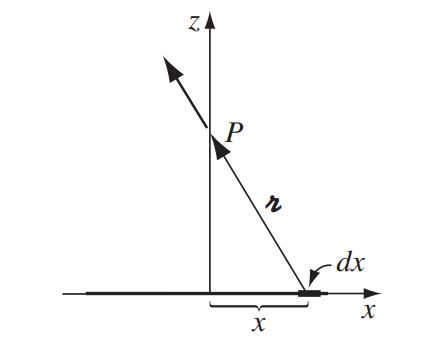
\includegraphics[height=6cm, width=6cm]{B.JPG}
        \\
        $
          \begin{cases}
            \overrightarrow{r}=L \hat{z}
            \\
            \\
            \overrightarrow{r}^'=x \hat{x}
            \\
            \\
            \overrightarrow{\scriptr}=r-r^'=L \hat{z}-x \hat{x}
            \\
            \\
            |\overrightarrow{\scriptr}|=\sqrt{L^2+x^2}
            \\
            \\
            \hat{\scriptr}=\dfrac{\overrightarrow{\scriptr}}{\scriptr}=\dfrac{L \hat{z}}{\sqrt{L^2+x^2}}
          \end{cases}
          \\
          \\
          \\
          F=QE \longrightarrow E=\dfrac{E}{Q}=\dfrac{1}{Q} \dfrac{1}{4 \pi \epsilon_0} \dfrac{Q q_{source}}{\scriptr^2}
          \\
          \\
          \therefore ~~~ |\overrightarrow{E}|=\dfrac{1}{4 \pi \epsilon_0} \dfrac{q_{source}}{\scriptr^2}
          \\
          \\
        $
        So with this fact, let's continue the work
        $
          \\
          \\
          \\
          \overrightarrow{E}=\dfrac{1}{4 \pi \epsilon_0} \bigints\limits_{0}^{x} \dfrac{\lambda}{\scriptr^2} \hat{\scriptr} dx
          =\dfrac{1}{4 \pi \epsilon_0} \bigints\limits_{0}^{x} \dfrac{\lambda}{x^2+L^2} \dfrac{L \hat{z}}{\sqrt{L^2+x^2}} dx
          \\
          \\
          \\
          =\dfrac{\lambda}{4 \pi \epsilon_0} \left[
            \bigints\limits_{0}^{x} \dfrac{L \hat{z}}{\left(L^2+x^2\right)^{3/2}}
            -\bigints\limits_{0}^{x} \dfrac{x \hat{x}}{\left(L^2+x^2\right)^{3/2}}
          \right]
          \\
          \\
          \\
          \begin{cases}
            (A): x=L tan(\theta), ~~~ \theta=arctan(\dfrac{x}{L})
            \\
            \\
            (B): k=L^2+x^2
          \end{cases}
          \\
          \\
          \\
          =\dfrac{\lambda}{4 \pi \epsilon_0} \left[
            L^2 \bigints\limits_{0}^{arctan(\dfrac{x}{L})} \dfrac{sec^2(\theta)}{L^3 sec^3(\theta)} \hat{z} d\theta
            -\bigints\limits_{L^2}^{L^2+x^2} \dfrac{\hat{x}}{2 k^{\dfrac{3}{2}}} dk
          \right]
          \\
          \\
          \\
          =\dfrac{\lambda}{4 \pi \epsilon_0} \left[
            \dfrac{L-\sqrt{L^2+x^2}}{L \sqrt{L^2+x^2}} \hat{x}
            +\dfrac{x}{L \sqrt{L^2+x^2}} \hat{z}
          \right]
          \\
          \\
          \\
          \therefore ~~~ \overrightarrow{E}=\dfrac{\lambda}{4 \pi \epsilon_0} \left[
            \dfrac{L-\sqrt{L^2+x^2}}{L \sqrt{L^2+x^2}} \hat{x}
            +\dfrac{x}{L \sqrt{L^2+x^2}} \hat{z}
          \right] ~~~ \checkmark
        $
      }

    \item Let the electric field, expressed in spherical coordinates, be
    $$\overrightarrow{E}(\overrightarrow{r})=\dfrac{b}{r}\hat{r}
    +\dfrac{2b}{3r} sin(\theta) cos(\theta) sin(\phi) \hat{\theta}
    +\dfrac{b}{3r} sin(\theta) cos(\phi) \hat{\phi}$$
    where $b$ is some constant. Find the charge density $\rho(r, \theta, \phi)$.

      \textcolor{hwColor}{
        One page 70 of the textbook we have $\overrightarrow{\nabla}.\overrightarrow{E}=\dfrac{1}{\epsilon_0} \rho$. Therefore,
        \\
        \\
        $
          \overrightarrow{\nabla}.a
          =\dfrac{1}{r^2} \dfrac{\partial}{\partial r} (r^2 a_r)
          +\dfrac{1}{r sin(\theta)} \dfrac{\partial}{\partial \theta} \left(sin(\theta) a_{\theta}\right)
          +\dfrac{1}{r sin(\theta)} \dfrac{\partial a_{\phi}}{\partial \phi}
          \\
          \\
          \\
          \rho=\epsilon_0 \left(\overrightarrow{\nabla}.\overrightarrow{E}\right)
          \\
          \\
          =\epsilon_0 \dfrac{1}{r^2} \dfrac{\partial}{\partial r} (r^2 \dfrac{b}{r})
          +\dfrac{1}{r sin(\theta)} \dfrac{\partial}{\partial \theta} \left(sin(\theta) \dfrac{2b}{3r} sin(\theta) cos(\theta) sin(\phi) \right)
          +\dfrac{1}{r sin(\theta)} \dfrac{\partial \dfrac{b}{3r} sin(\theta) cos(\phi)}{\partial \phi}
          \\
          \\
          \\
          =\epsilon_0 \left[
            \dfrac{b}{r^2} \partial_r(r)+\partial_{\theta}\left(sin^2(\theta) cos(\theta)\right) \left(\dfrac{2b sin(\theta)}{3 r^2 sin(\theta)}\right)+\dfrac{b}{3r^2} \partial_{\phi}\left(cos(\phi)\right)
          \right]
          \\
          \\
          \\
          =\epsilon_0 \left[
            \dfrac{b}{r^2}-\dfrac{2b sin(\phi)}{3 r^2 sin(\theta)} \left(2 sin(\theta) cos^2(\theta)-sin^3(\theta)\right)-\dfrac{b sin(\phi)}{3r^2}
          \right]
          \\
          \\
          \\
          =\epsilon_0 \left[
            \dfrac{b}{r^2} \left[1-\dfrac{sin(\phi)}{3}+\dfrac{4 cos^2(\theta) sin(\phi)}{3}-\dfrac{2 sin(\phi) sin^2(\theta)}{3}\right]
          \right]
          \\
          \\
          \\
          \therefore ~~~ \rho(r, \theta, \phi)=\epsilon_0 \dfrac{b}{r^2} \left[
            1+\dfrac{2sin(\phi)}{3} \left(2 cos^2(\theta)-sin^2(\theta)-\dfrac{1}{2}\right)
          \right] ~~~ \checkmark
        $
      }

    \item Look up the mass and charge of a proton and the values of the appropriate constants for this problem.
    \begin{enumerate}
      \item For a given separation $r$ between two protons, calculate the ratio
      of the magnitude of their electric repulsion to the magnitude of
      their gravitational attraction. That is why gravity is known as a
      weak force.

        % \textcolor{hwColor}{
        
        % }

      \item Two protons in a helium nucleus are roughly $10^{-15}m$ apart. Calculate the force of 
      electric repulsion in Newtons. To put that in perspective, calculate the acceleration (in $m/s^2$) that a proton
      would feel. That is why the nuclear force that overcomes this repulsion is known as the strong force.

        % \textcolor{hwColor}{
        
        % }

    \end{enumerate}

  \end{enumerate}

\end{document}